%review=doublespace preprint=single 5p=2 column
\documentclass[12pt,3p,authoryear]{elsarticle}

%% add packages %%
%% ------------ %%
\usepackage[hyphens]{url}
\usepackage{graphicx}
\usepackage{booktabs}
\usepackage[T1]{fontenc}
\usepackage{lmodern}
\usepackage{caption}
\usepackage{subfig}
\usepackage{amssymb, amsmath}
\usepackage[inline]{enumitem}
\usepackage{float}
\usepackage{tabularx}
\usepackage[dvipsnames, table]{xcolor}
\usepackage{ifxetex, ifluatex}
\usepackage{fixltx2e}
\usepackage[unicode=true, colorlinks]{hyperref}
\usepackage{cleveref}
\usepackage{tabu}
\usepackage{mathpazo}
%% ------------ %%

%% Conditional Packages %%
%% -------------------- %%

\usepackage{easyReview}



% use upquote if available, for straight quotes in verbatim environments
\IfFileExists{upquote.sty}{\usepackage{upquote}}{}

\ifnum 0\ifxetex 1\fi\ifluatex 1\fi=0 % if pdftex
  \usepackage[utf8]{inputenc}


\else % if luatex or xelatex
  \usepackage{fontspec}
  \ifxetex
    \usepackage{xltxtra,xunicode}
  \fi
  \defaultfontfeatures{Mapping=tex-text,Scale=MatchLowercase}
  \newcommand{\euro}{€}



    \setmonofont{sourcecodepro}


\fi

% use microtype if available
\IfFileExists{microtype.sty}{\usepackage{microtype}}{}






\usepackage{longtable}




% Pandoc toggle for numbering sections (defaults to be off)
\setcounter{secnumdepth}{5}

%% Use Landscape Pages
\usepackage{lscape}

\usepackage{setspace}
\setstretch{1.5}

\usepackage{lmodern}

%% -------------------- %%

%% Create and Provide some customizations %%
%% -------------------------------------- %%
\providecommand{\tightlist}{%
  \setlength{\itemsep}{0pt}\setlength{\parskip}{0pt}}
  
%% Custom macros
\newtheorem{mydef}{Definition}
\newcommand{\bs}[1]{\ensuremath{\boldsymbol{#1}}}
\newcommand{\diag}[1]{\mathrm{diag}\left(#1\right)}
\newcommand{\seq}[3][1]{\ensuremath{#2_{#1},\ldots,\,#2_{#3}}}
\newcommand{\note}[1]{\marginpar{\scriptsize\tt{\color{RoyalBlue}#1}}}
\newcommand{\edit}[1]{{\color{OrangeRed} #1}}

%% Declare Operators
\newcommand{\argmin}{\operatornamewithlimits{arg\,min}}
\newcommand{\argmax}{\operatornamewithlimits{arg\,max}}

% set some lengths
\setlength{\parindent}{0pt}
% \setlength{\parskip}{6pt plus 2pt minus 1pt}
\setlength{\emergencystretch}{3em}  % prevent overfull lines

%% Hyperref color setup
\AtBeginDocument{%
  %% Define Colors
  \newcommand\myshade{80}
  \colorlet{mylinkcolor}{violet!\myshade!black}
  \colorlet{mycitecolor}{YellowOrange!\myshade!black}
  \colorlet{myurlcolor}{Aquamarine!\myshade!black}

  \hypersetup{
    breaklinks = true,
    bookmarks  = true,
    pdfauthor  = {},
    pdftitle   = {Comparison of Multivariate Estimation Methods},
    linkcolor  = mylinkcolor,
    citecolor  = mycitecolor,
    urlcolor   = myurlcolor,
    colorlinks = true,
  }
}
\urlstyle{same}  % don't use monospace font for urls
%% -------------------------------------- %%

%% Customizations %%
%% -------------- %%
 % turn line numbering on

%% -------------- %%

%% Configure Bibliography %%
%% ---------------------- %%
\bibliographystyle{elsarticle-harv}
\biboptions{numbers,sort&compress}

\makeatletter
\providecommand{\doi}[1]{%
  \begingroup
    \let\bibinfo\@secondoftwo
    \urlstyle{rm}%
    \href{http://dx.doi.org/#1}{%
      doi:\discretionary{}{}{}%
      \nolinkurl{#1}%
    }%
  \endgroup
}
\makeatother

% 

%% Header Includes %%
%% --------------- %%
%% --------------- %%



\begin{document}
%% --- Front Matter Start --- %%
\begin{frontmatter}

  \title{Comparison of Multivariate Estimation Methods}
  
    \author[KBM]{Raju Rimal\corref{c1}}
   \ead{raju.rimal@nmbu.no} 
   \cortext[c1]{Corresponding Author}
    \author[KBM]{Trygve Almøy}
   \ead{trygve.almoy@nmbu.no} 
  
    \author[NMBU]{Solve Sæbø}
   \ead{solve.sabo@nmbu.no} 
  
      \address[KBM]{Faculty of Chemistry and Bioinformatics, Norwegian University of Life
Sciences, Ås, Norway}
    \address[NMBU]{Prorector, Norwegian University of Life Sciences, Ås, Norway}
  
  \begin{abstract}
  Prediction performance often does not reflect the estimation behaviour
  of a method. High error in estimation not necessarily results in high
  prediction error but can lead to an unreliable prediction when test data
  are in a different direction than the training data. In addition, the
  effect of a variable becomes unstable and can not be interpreted in such
  situations. Many research fields are more interested in these estimates
  than performing prediction. This study compares some newly-developed
  (envelope) and well-established (PLS, PCR) prediction methods using
  simulated data with specifically designed properties such as
  multicollinearity, the correlation between multiple responses and
  position of principal components of predictor that are relevant for the
  response. This study aims to give some insight into these methods and
  help the researcher to understand and use them for further study.
  \emph{Write some specifics from the results to show what we have found.}
  \end{abstract}
   \begin{keyword} model-comparison,multi-response,simrel,estimation,estimation error,meta modeling\end{keyword}

\end{frontmatter}

\section{Introduction}\label{introduction}

Estimation of parameters in a regression model is an integral part of
many research study. Research fields such as social science,
econometrics, psychology and medical study are more interested in
measuring the impact of certain indicator or variable rather than
performing prediction. Such studies have a large influence on people's
perception and also help in policy making and decisions.

Technology has facilitated researcher to collect a large amount of data
however often times, such data either contains irrelevant information or
are highly collinear. Researchers are devising new estimators to extract
information and identify their inter-relationship. Some estimators are
robust towards fixing the multicollinearity problem while some are
targeted to model only the relevant information contained in the
response variable.

This study extends the \citep{rimal2019pred} and compares some
well-established estimators such as Principal Components Analysis (PCA),
Partial Least Squares (PLS) together with two new methods based on
envelope estimation: Envelope estimation in predictor space (Xenv)
\citep{cook2010envelope} and simultaneous estimation of envelope (Senv)
\citep{cook2015simultaneous}. The estimation process of these methods is
discussed in {[}Methods{]} section. The comparison tests the estimation
performance of these methods using multi-response simulated data from a
linear model with controlled properties. The properties include the
number of predictors, level of multicollinearity, the correlation
between different response variables and the position of relevant
predictor components. These properties are explained in
\protect\hyperlink{experimental-design}{Experimental Design} section
together with the strategy behind the simulation and data model.

\section{Simulation Model}\label{simulation-model}

\begin{itemize}
\tightlist
\item
  Reduction of the regression model
\item
  Include the figure from previous paper
\item
  How the covariance and coefficients are related
\item
  From the construction of the covariance matrix of latent variables to
  the simulated data
\item
  How and what simulation parameters are related to properties of data
\end{itemize}

\section{Estimation Methods}\label{estimation-methods}

A regression model is written as,

\begin{equation}
\underset{(1\times m)}{\mathbf{y}} =
  \underset{(1\times p)(p\times m)}
    {\mathbf{x}\boldsymbol{\beta}} +
  \underset{(1 \times m)}{\boldsymbol{\varepsilon}}
\label{eq:reg-model}
\end{equation}

where \(\mathbf{y}\) is a vector of \(m\) responses measured about their
means, \(\mathbf{x}\) is a vector of \(p\) predictors measured about
their means, \(\boldsymbol{\beta}\) is a matrix of regression
coefficients and \(\boldsymbol{\varepsilon}\) is a vector of independent
error terms with constant variance \(\boldsymbol{\Sigma}_{y|x}\). In
ordinary least squares, coefficient \(\boldsymbol{\beta}\) is estimated
as,

\begin{equation}
\underset{(p\times m)}{\boldsymbol{\hat{\beta}}} =
  \left(\underset{(p\times n)}{\mathbf{x}^t}
  \underset{(n\times p)}{\mathbf{x}}\right)^{-1}
  \underset{(p \times n)(n \times m)}{\mathbf{x}^t\mathbf{y}}
\label{eq:reg-beta}
\end{equation}

\subsection{Principal Components
Regression}\label{principal-components-regression}

Principal Components are new set of variables from the transformation of
original dataset such that they are uncorrelated with each other and the
variation in the original data are ordered from first to last of these
new variables. Let us define a transformation of \(\mathbf{x}\) as,

\begin{equation}
\underset{(1\times p)}{\mathbf{x}} =
  \underset{(1 \times k)}{\mathbf{z}}
  \underset{(k \times p)}{\mathbf{R}^t}
\label{eq:x2z}
\end{equation}

where \(\mathbf{R}\) is the eigenvectors corresponding to the covariance
of \(\mathbf{x}\) and \(\mathbf{z}\) are the principal components. A
regression model can be defined in terms of \(\mathbf{z}\) as,

\begin{equation}
\underset{(1 \times m)}{\mathbf{y}} =
  \underset{(1 \times k)}{\mathbf{z}}
    \underset{(k \times m)}{\boldsymbol{\alpha}} +
  \underset{(1 \times m)}{\boldsymbol{\varepsilon}}
\label{eq:latent-model}
\end{equation}

Since the variation is ordered in \(z\), only \(k\le p\) columns of
\(z\) are used so that \(p-k\) uninformative components are not used for
modeling. The regression coefficient of \eqref{eq:latent-model} can be
estimated as,

\begin{equation}
\underset{(k\times m)}{\boldsymbol{\hat{\alpha}}} =
  \left(\underset{(k \times n)}{\mathbf{z}^t}
    \underset{(n \times k)}{\mathbf{z}}\right)^{-1}
  \underset{(k \times n)(n \times m)}{\mathbf{z}^t\mathbf{y}}
\label{eq:reg-alpha}
\end{equation}

Using \eqref{eq:x2z} in \eqref{eq:reg-beta}, we get,

\[
\begin{aligned}
\underset{(p\times m)}{\boldsymbol{\hat{\beta}}} =
  \left[
    \underset{(p\times k)(k \times n)}{\mathbf{R}\mathbf{z}^t}
    \underset{(n\times k)(k \times p)}{\mathbf{z} \mathbf{R}^t}
  \right]^{-1}
  \underset{(p\times k)(k \times n)}{\mathbf{R}\mathbf{z}^t}
  \underset{(n\times m)}{y}
\end{aligned}
\]

\subsection{Partial Least Squares
Regression}\label{partial-least-squares-regression}

\begin{itemize}
\tightlist
\item
  How beta coefficients are constructed
\item
  How it is dependent on the variance-covariance matrices
\item
  In what way PLS1 and PLS2 differ
\end{itemize}

\subsection{Envelope Estimations}\label{envelope-estimations}

\begin{itemize}
\tightlist
\item
  How beta coefficients are constructed
\item
  How it is dependent on the variance-covariance matrices
\item
  In what way Xenv and Senv differ
\end{itemize}

\hypertarget{experimental-design}{\section{Experimental
Design}\label{experimental-design}}

An R \citep{coreR2018} package \texttt{simrel}
\citep{Rimal2018, saebo2015simrel} is used to simulate data. For the
simulation the number of observation is kept fixed at \(n = 100\) and
following four simulation parameters are used to obtain the data with
wide range of properties.

\begin{description}
\tightlist
\item[\textbf{Number of predictors:}]
In order to cover both tall \((n>p)\) and wide \((p>n)\) cases, \(p=20\)
and \(p=250\) number of predictors are simulated.
\item[\textbf{Multicollinearity in predictor variables:}]
A parameter \texttt{gamma} \((\gamma)\) in simulation controls the
exponential decline of eigenvalues \((\lambda_i, i = 1, \ldots p)\)
corresponding to predictor variables as,

\begin{equation}
  \lambda_i = e^{-\gamma(i-1)}, \gamma > 0 \text{ and } i = 1, 2, \ldots p
  \label{eq:gamma}
  \end{equation}

Two levels 0.2 and 0.8 of \texttt{gamma} are used for simulation so that
level 0.2 simulates the data with low multicollinearity and 0.8
simulates the data with high multicollinearity.
\item[\textbf{Position of relevant components:}]
Initial principal components of a non-singular covariance matrix are
larger than the later one. If the principal components corresponding to
predictors with larger variation is not relevant for a response, this
will just increase noise in the model. Here we will use two different
levels of position index of predictor components: a) 1, 2, 3, 4 and b)
5, 6, 7, 8. Predictor components irrelevant for a response makes
prediction difficult \citep{Helland1994b}. When combined with
multicollinearity, this factor can create both easy and difficult model
for both estimation and prediction.
\item[\textbf{Correlation in response variables:}]
Many estimators also uses the structure of response for their
estimation. Here the correlation between the responses are varied
through a simulation parameter \texttt{eta} \((\eta)\). The parameter
controls the exponential decline of eigenvalues
\(\kappa_j, j = 1, \ldots m (\text{ number of responses})\)
corresponding to response variables as,

\begin{equation}
\eta_i = e^{-\kappa(j-1)}, \kappa > 0 \text{ and } j = 1, 2, \ldots m
\label{eq:eta}
\end{equation}

Four levels 0, 0.4, 0.8 and 1.2 of \texttt{eta} are used in the so that
level 0 simulates the data with uncorrelated response variables while
1.2 simulates the highly correlated response variables.
\end{description}

\begin{figure}[!htb]
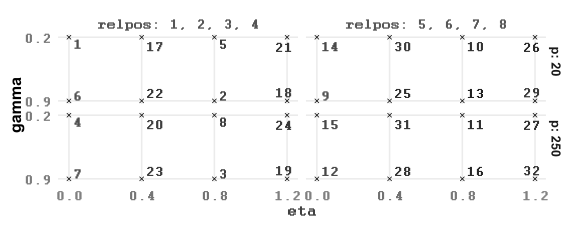
\includegraphics[width=1\linewidth]{main_files/figure-latex/design-plot-1} \caption{Experimental Design of simulation parameters. Each point represents an unique data property.}\label{fig:design-plot}
\end{figure}

Here we have assumed that there is only one informative response
component. In the final dataset, all predictors together span the same
space as the relevant predictor components and all response together
span the same space as the one informative response component. In
addition, coefficient of determination is fixed at 0.8 for all dataset.

A complete factorial design is adopted using different levels of factors
discussed above to create 32 design (Figure \ref{fig:design-plot}) each
of which gives dataset with unique properties. From each of these design
and each estimation method, 50 different datasets are simulated so that
each of them have same true population structure. In total,
\(5 \times 32 \times 50\) i.e., 8000 datasets are simulated.






\begin{figure}
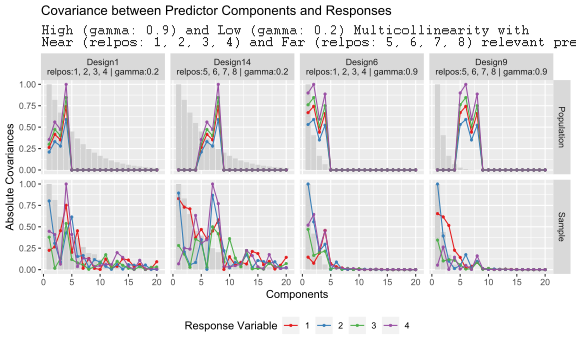
\includegraphics[width=1\linewidth]{main_files/figure-latex/cov-plot-1} \caption{Covariance between predictor components and response
variables in population (top) and in the simulated data (bottom) for
four different designs. The Bar in the background represents the
variance of corresponding components.}\label{fig:cov-plot}
\end{figure}

The simulation properties are directly reflected in the simulated data.
For example, in Figure \ref{fig:cov-plot}, design pairs at columns 1, 2
and 3, 4 differs their properties only in terms of relevant predictor
components while the design pairs at columns 1, 3 and 2, 4 differs only
in-terms of level of multicollinearity. The properties in population are
also reflected in the simulated samples.

\emph{\alert{May be we need to write few thing on how easy or difficult data are simulated with the interaction of these properties}}

\section{Basis of Comparison}\label{basis-of-comparison}

The focus of this study is to extend the exploration of
\citet{rimal2019pred} to estimative performance of PCR, PLS1, PLS2, Xenv
and Senv methods. The performance is measured on the basis of,

\begin{enumerate}
\def\labelenumi{\alph{enumi})}
\tightlist
\item
  average estimation error of a method using arbitrary number of
  components
\item
  average number of components used by a method to give minimum
  estimation error
\end{enumerate}

Let us define the expected estimation error as,

\begin{equation}
\mathcal{EE}_{ijkl} =
  \mathsf{E}{\left[\left(\boldsymbol{\beta}_{ij} -
  \boldsymbol{\hat{\beta}_{ijkl}}\right)^t
  \left(\boldsymbol{\beta}_{ij} - \boldsymbol{\hat{\beta}_{ijkl}}\right)\right]}
\label{eq:est-error}
\end{equation}

for response \(j = 1, \ldots 4\) in a given design \(i=1, 2, \ldots 32\)
and method \(k=1(PCR), \ldots 5(Senv)\) using \(l=0, \ldots 10\) number
of components. Since both the expectation and the variance of
\(\hat{\boldsymbol{\beta}}\) are unknown, the prediction error are
estimated using data from 50 replications as follows,

\begin{equation}
\widehat{\mathcal{EE}_{ijkl}} =
  \sum_{r=0}^{50}{\left[\left(\boldsymbol{\beta}_{ij} -
  \boldsymbol{\hat{\beta}_{ijklr}}\right)^t
  \left(\boldsymbol{\beta}_{ij} - \boldsymbol{\hat{\beta}_{ijklr}}\right)\right]}
\label{eq:estimated-est-error}
\end{equation}

where, \(\widehat{\mathcal{EE}_{ijkl}}\) is the estimated prediction
error averaged over \(r=50\) replicates.

\section{Exploration}\label{exploration}





\begin{figure}[!htb]
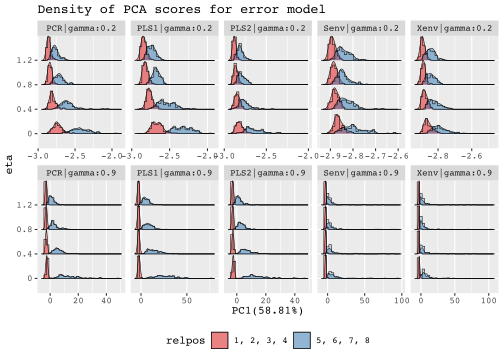
\includegraphics[width=1\linewidth]{main_files/figure-latex/est-pca-hist-mthd-gamma-relpos-1} \caption{Scores density corresponding to first principal component
of \emph{error dataset} (\(\mathbf{u}\)) subdivided by \texttt{methods},
\texttt{gamma} and \texttt{eta} and grouped by \texttt{relpos}.}\label{fig:est-pca-hist-mthd-gamma-relpos}
\end{figure}






\begin{figure}[!htb]
\includegraphics[width=1\linewidth]{main_files/figure-latex/comp-pca-hist-mthd-gamma-relpos-1} \caption{Score density corresponding to first principal component
of \emph{component dataset} (\(\mathbf{v}\)) subdivided by
\texttt{methods}, \texttt{gamma} and \texttt{eta} and grouped by
\texttt{relpos}.}\label{fig:comp-pca-hist-mthd-gamma-relpos}
\end{figure}

\begin{itemize}
\tightlist
\item
  A similar exploration as previous paper but can be different in case
  of new idea
\end{itemize}

\subsection{Dataset for Analysis}\label{dataset-for-analysis}

\begin{itemize}
\tightlist
\item
  Preparation of dataset for MANOVA analysis (i.e.~minimum estimation
  error using arbitrary number of components)
\item
  A component dataset is also created for testing the use of components
  by each of these methods
\end{itemize}

\subsection{Regression Coefficients}\label{regression-coefficients}

\begin{itemize}
\tightlist
\item
  In case of some idea on comparing regression coefficients through some
  statistical way, this can be included here
\item
  Otherwise can also be done just by using plots
\end{itemize}

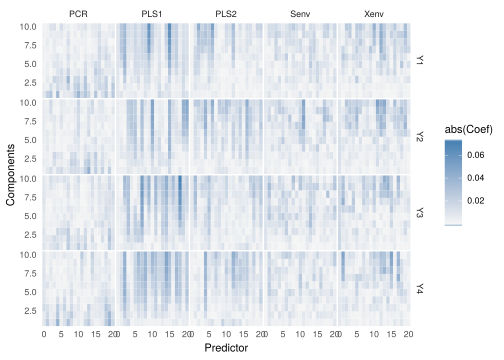
\includegraphics[width=1\linewidth]{main_files/figure-latex/unnamed-chunk-2-1}

\subsection{Prediction and Estimation
Error}\label{prediction-and-estimation-error}

\begin{itemize}
\tightlist
\item
  Explore both estimation error and number of components and try to bind
  them with the prediction error for the similar case
\end{itemize}

\section{Analysis}\label{analysis}





\begin{figure}
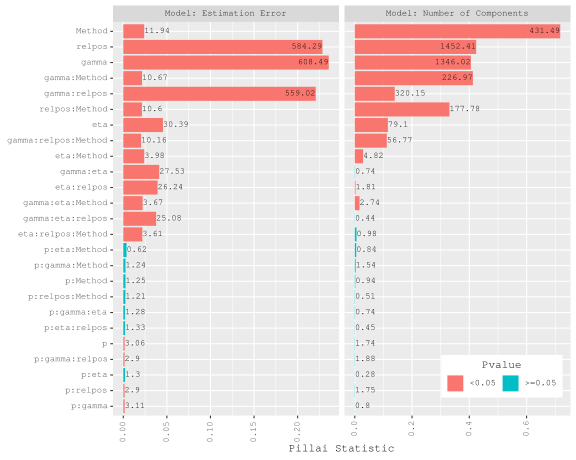
\includegraphics[width=1\linewidth]{main_files/figure-latex/manova-plot-1} \caption{Pillai Statistic and F-value for the MANOVA model. The
bar represents the Pillai Statistic and the text labels are F-value for
corresponding factor.}\label{fig:manova-plot}
\end{figure}

\begin{itemize}
\tightlist
\item
  A MANOVA model is fitted using the dataset prepared in previous
  section
\end{itemize}

\subsection{Error Analysis}\label{error-analysis}




\begin{figure}
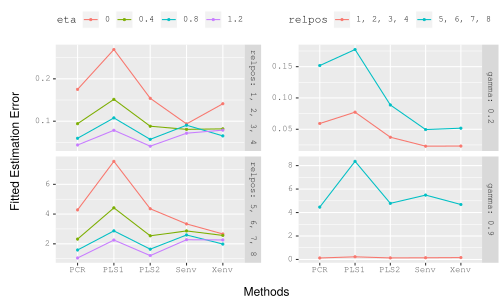
\includegraphics[width=1\linewidth]{main_files/figure-latex/est-eff-plots-1} \caption{Effect plot of some interactions of the multivariate
linear model of estimation error}\label{fig:est-eff-plots}
\end{figure}

\begin{itemize}
\tightlist
\item
  Effect analysis of estimation error model
\item
  Tie up these results with prediction error in previous paper
\end{itemize}

\subsection{Component Analysis}\label{component-analysis}




\begin{figure}[!htb]
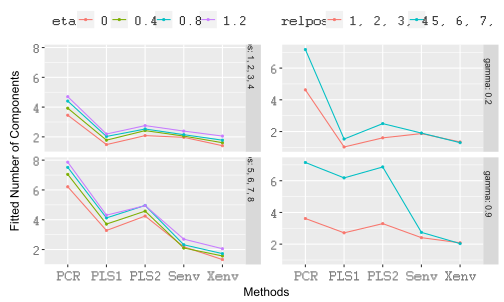
\includegraphics[width=1\linewidth]{main_files/figure-latex/comp-eff-plots-1} \caption{Effect plot of some interactions of the multivariate
linear model of number of components to get minimum prediction error}\label{fig:comp-eff-plots}
\end{figure}

\begin{itemize}
\tightlist
\item
  Effect analysis of number of component model
\item
  Tie up these results in previous paper
\end{itemize}

\section{Discussion and Conclusion}\label{discussion-and-conclusion}

\begin{itemize}
\tightlist
\item
  A similar discussion but based more on why the methods worked in the
  way we have seen in the results in previous sections
\item
  Some concluding remarks and limitations (or a gate for further
  exploration)
\end{itemize}


\renewcommand\refname{References}
\bibliography{ref-db.bib}


\end{document}
